\documentclass[tikz,border=5pt]{standalone}
\begin{document}
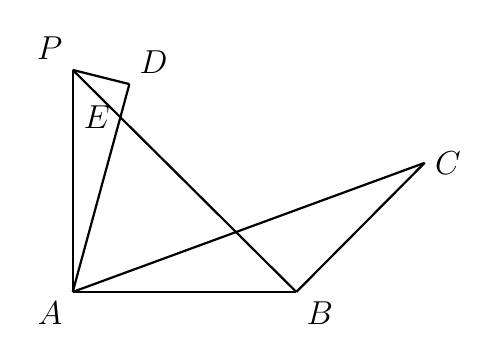
\begin{tikzpicture}[thick, font=\large, scale=1]
  % 坐标点
  \coordinate (A) at (0,0);
  \coordinate (B) at (2.84,0);
  \coordinate (C) at (4.47,1.64);
  \coordinate (P) at (0,2.82);
  \coordinate (D) at (0.72,2.64);
  \coordinate (E) at (0.605,2.219);

  % 线段（已删除线段 CD 的笔画）
  \draw (A) -- (B);
  \draw (B) -- (C);
  \draw (A) -- (C);
  \draw (A) -- (P);
  \draw (P) -- (D);
  \draw (P) -- (B);
  \draw (A) -- (D);

  % 标签
  \node[above left]  at (P) {$P$};
  \node[above right] at (D) {$D$};
  \node[left]        at (E) {$E$};
  \node[right]       at (C) {$C$};
  \node[below left]  at (A) {$A$};
  \node[below right] at (B) {$B$};
\end{tikzpicture}
\end{document}
